\documentclass{beamer}
%\usecolortheme{dove} %Make title black
\usepackage{graphicx} % Allows including images
\usepackage{booktabs} % Allows the use of \toprule, \midrule and \bottomrule in tables
%\usepackage{siunitx}  %Use SI unit formatting
%\sisetup{range-phrase=--}
%Bold command
%\newcommand\SEC[1]{\textbf{\uppercase{#1}}}
\usepackage{pifont}% http://ctan.org/pkg/pifont
\newcommand{\cmark}{\ding{51}}%
\newcommand{\xmark}{\ding{55}}%
%\usepackage{siunitx}  %Use SI unit formatting
%For drawing beam line
\include{tikz}
\usetikzlibrary{shapes.misc}
\usetikzlibrary{shapes,arrows,decorations.markings,shadows,positioning}
%Adjust width of slide
\newcommand\Wider[2][3em]{%
	\makebox[\linewidth][c]{%
		\begin{minipage}{\dimexpr\textwidth+#1\relax}
			\raggedright#2
		\end{minipage}%
	}%
}

\include{header}
\usebackgroundtemplate{
\includegraphics[width=\paperwidth]{NormalANLMaroon.pdf}}
\title[PSI Talk]{Optimization of the AWA Drive Linac}
\author[Speaker]{Nicole Neveu}
\subtitle{}
\institute[ANL/IIT]{Argonne National Laboratory\\Illinois Institute of Technology}
\date{\today}

\logo{%
	\makebox[0.95\paperwidth]{%
		%\includegraphics[width=3cm,keepaspectratio]{IIT_logo}%
		\hfill%
		\includegraphics[width=3cm,keepaspectratio]{IIT_logo_blk}%
	}%
}

\setbeamertemplate{navigation symbols}{}


%------------------------------------------------------
\begin{document}
\setbeamertemplate{footline}{}
{
	\usebackgroundtemplate{
\includegraphics[width=\paperwidth]{TitleANLMaroon}}
	\logo{%
		\makebox[0.95\paperwidth]{%
			\includegraphics[width=3cm,keepaspectratio]{IIT_logo}%
			\hfill%
			%\includegraphics[width=3cm,keepaspectratio]{IIT_logo_blk}%
		}%
	}
	\frame{\titlepage}
}

\setbeamertemplate{footline}[page number]{}	
	
% FRAME: overview
\begin{frame}
  \frametitle{Outline}
  \tableofcontents
\end{frame}
% ========================================
% main slides come here
% ========================================
\section{Optimization Introduction}
%\begin{frame}
%  \frametitle{Before we start ...}
%\end{frame}

\begin{frame}[plain]
\frametitle{Optimization Introduction}

\Wider[4em]{
  \setlength{\leftmargin}{0.1cm}
  \begin{itemize}
    \item{Why use optimization?}\\
    \begin{itemize}
      %\item{\underline{\textbf{Drive Line}}: $Cs_2Te$ cathode, 6 linac cavities}
      \item{Reduce the number of simulations needed}
      \begin{itemize}
        \item{Eliminate brute force simulations}
        \item{i.e. scanning parameters one by one}
        \item{This is not efficient when many variables can change} \\
      \end{itemize} 
      %\item{\underline{\textbf{Witness Line}}: $Mg$ cathode, 1 lin}
      \item{Get better beam parameters} \\
      \item{Try to understand the parameter space better}
    \end{itemize}
\end{itemize}

}
\end{frame}

\begin{frame}
\frametitle{Optimization Introduction}
So, what is an optimization algorithm?
\begin{itemize}
	\item{Similar to coding definition of algorithm.} 
	\item{Set of rules that determines which points are good based on math. 
	Each point is compared to other points, and you have to pick what you want to optimize.}
	\item{What you want to optimize = "objectives"}
	\begin{itemize}
	\item{in optimization terminology}
	\end{itemize}
	\item{Genetic Algorithms are commonly used in accelerator physics}
	\begin{itemize}
		\item{Gwanghui, Borland, OPAL people, etc.}
	\end{itemize}
\end{itemize}

\end{frame}
%--------------------------------------------------------------------------------------------
\section{Types of Optimization Algorithms}
\begin{frame}
  \frametitle{Genetic Algorithms}
  \begin{itemize}
    \item{Based on biology and nature}
    \item{This method is close to random sampling (IMO)}
    \item{In general the steps are:}
    \begin{enumerate}
    	\item{Do initial random sample, this is initial "population"}
    	\item{Choose best points w.r.t objectives}
    	\item{"Breed" best points (mix their input parameters)}
    	\item{Do another set of simulations with the new "generation"}
    	\item{Repeat for many generations } 	
    \end{enumerate}
	\end{itemize}
\vspace*{-\baselineskip}
\begin{center}
	\includegraphics[width=0.5\textwidth]{ga}
\end{center}
\end{frame}

\begin{frame}
	\frametitle{Model Based Algorithms}
			\begin{itemize}
			\item These methods try to use information about the problem instead of random sampling.
			\item For the IPAC paper, we used a method called BOBYQA:
			\begin{itemize}
				\item Bounded Optimization BY Quadratic Approximation
				\begin{enumerate}
					\item The initial sample is N+1 points (where N is number of variables)
					\item The objectives are found for those points
					\item A quadratic is built using the objective values
					\item The next point is chosen by trying to minimize the objective
					\item This process is repeated until convergence criteria met
				\end{enumerate}
				
				\item Let's look at an AWA example....
			\end{itemize}
		\end{itemize}
	\vspace*{-\baselineskip}
	\begin{center}
		\includegraphics[width=0.5\textwidth]{bobyqa}
	\end{center}
\end{frame}

%--------------------------------------------------------------------------------------------
\section{Initial OPAL and Python Optimization Results}
\begin{frame}
	\frametitle{Initial Optimization Work (Linac only)}
	\Wider[4em]{
	  \begin{minipage}{0.6\textwidth}
	  \begin{itemize}
	  	\item{Determine what emittance and bunch length we can expect from the linac}
	  	\item{Understand beam at entrance of quads}
	  	\begin{itemize}
	  		\item After $L_6$: $z_1=12.51$ m
	  	\end{itemize}
	  	\item{Used pre-packaged algorithm BOBYQA}
	  	\item{Varied 10 parameters:}
	  \end{itemize}
	  \end{minipage}%
	  \begin{minipage}{0.4\textwidth}
		\def \gunleft {-1.0}
		\def \gunright {0.3}
		\def \loneright {1.0}
		\def \ltworight {2.0}
		\def \lthreeright {3.0}
		\def \lfourright {4.0}
		\def \lfiveright {5.0}
		\def \lsixright {6.0}
		\centering
		\begin{center}
		\begin{tikzpicture}[scale=0.55]%,use optics
		%Gun drawings
		\draw[fill=orange, very thick, rounded corners =0.1cm] (\gunleft,0.5)rectangle (\gunright,1.5) node[pos=.5, white] {\textbf{Gun}} ;
		
		%S1
		\node[] at (-1.3,2.9) {$S_1$};
		\draw[ultra thick, fill=black!60!green] (-1.4,-0.5)rectangle  (-1.0,0.5) node[pos=.5, white] {} ;
		\draw[black, ultra thick] (-1.4,-0.5) -- (-1.0,0.5);
		\draw[black, ultra thick] (-1.4,0.5) -- (-1.0,-0.5);
		\draw[ultra thick, fill=black!60!green] (-1.4,1.5)rectangle  (-1.0,2.5) node[pos=.5, white] {} ;
		\draw[black, ultra thick] (-1.4,1.5) -- (-1.0,2.5);
		\draw[black, ultra thick] (-1.4,2.5) -- (-1.0,1.5);
		%S2
		\node[] at (-0.8,2.9) {$S_2$};
		\draw[ultra thick, fill=black!60!green] (-1.0,-0.5)rectangle  (-0.6,0.5) node[pos=.5, white] {} ;
		\draw[black, ultra thick] (-1.0,-0.5) -- (-0.6,0.5);
		\draw[black, ultra thick] (-1.0,0.5) -- (-0.6,-0.5);
		\draw[ultra thick, fill=black!60!green] (-1.0,1.5)rectangle  (-0.6,2.5) node[pos=.5, white] {} ;
		\draw[black, ultra thick] (-1.0,1.5) -- (-0.6,2.5);
		\draw[black, ultra thick] (-1.0,2.5) -- (-0.6,1.5);
		
		%S3
		\node[] at (0.2,2.9) {$S_3$};
		\draw[ultra thick, fill=black!60!green] (-0.1,-0.5) rectangle  (0.3,0.5) node[pos=.5, white] {};
		\draw[black, ultra thick] (-0.1,-0.5) -- (0.3,0.5);
		\draw[black, ultra thick] (-0.1,0.5) -- (0.3,-0.5);
		\draw[ultra thick, fill=black!60!green] (-0.1,1.5) rectangle  (0.3,2.5) node[pos=.5, white] {};
		\draw[black, ultra thick] (-0.1,1.5) -- (0.3,2.5);
		\draw[black, ultra thick] (-0.1,2.5) -- (0.3,1.5);
		%Linac drawings 
		\draw[fill=blue, ultra thick, rounded corners =0.1cm] (\loneright,0)rectangle  ({\loneright+0.84},2) node[pos=.5, white] {$L_1$} ;
		\draw[fill=blue, ultra thick, rounded corners =0.1cm] (\ltworight,0)rectangle  ({\ltworight+0.84},2) node[pos=.5, white] {$L_2$};
		\draw[fill=blue, ultra thick, rounded corners =0.1cm] (\lthreeright,0)rectangle ({\lthreeright+0.84},2) node[pos=.5, white] {$L_3$};
		\draw[fill=blue, ultra thick, rounded corners =0.1cm] (\lfourright,0)rectangle ({\lfourright+0.84},2) node[pos=.5, white] {$L_4$};
		\draw[fill=blue, ultra thick, rounded corners =0.1cm] (\lfiveright,0)rectangle ({\lfiveright+0.84},2) node[pos=.5, white] {$L_5$};
		\draw[fill=blue, ultra thick, rounded corners =0.1cm] (\lsixright,0)rectangle ({\lsixright+0.84},2) node[pos=.5, white] {$L_6$};
		\end{tikzpicture}
	\end{center}
	\end{minipage}%
\begin{center}
\setcounter{mpfootnote}{\value{footnote}}%
\renewcommand{\thempfootnote}{\arabic{mpfootnote}}%	
\begin{tabular}{ l *{3}{c}}
	%\toprule
	\textbf{Variable} & \textbf{Range} & \textbf{Unit} \\
	\midrule
	Solenoid Strength & $ 0 \le S_3 \le 440$  & amps \\
	Phase of Gun & $-60 \le \phi_g \le 60$  & degrees \\
	Laser Radius  & $0.1 \le R \le 30$  & mm \\
	Laser FWHM  & $2 \le T \le $10  & ps \\
	Cavity Phase & $-20 \le \phi_L \le 20$\footnote[1]{$\phi_L=[\phi_{L_1},\ldots,\phi_{L_6}]$} & degrees
	%\bottomrule    
\end{tabular}
\end{center}
}
\end{frame}

\begin{frame}
	\frametitle{Linac Optimization}
	 \begin{itemize}
		  	\item{1,000 point sample was done}
		  	\item{132 simulations completed w/o error}
		  	\item{Scaled and shifted raw values to remove unit dependence}
	 \end{itemize}
	 \begin{align*}
	 \bar{\epsilon}_x (v,z_1) = \frac{ \epsilon_x (v,z_1) - \epsilon_{\min} } { \epsilon_{\max} - \epsilon_{\min} }
	 \end{align*}
	 
	 \begin{itemize}
	  	\item{Used 11 weights from 0-1}
	  	\item Code: w = np.arange(0, 1.1, 0.1)
	\end{itemize}
\end{frame}

\begin{frame}
	\frametitle{Linac Optimization}
	\begin{itemize}
		\item{Solved 11 optimization problems $f(v,w)$ using BOBYQA}
		\item i.e. The minimum f(v,w) values were used as starting points for BOBYQA optimization runs.
		\item v = 10 optimization variable from table below 
	\end{itemize}	
	\begin{gather*}
	w\in\left\{ 0, 0.1, \ldots, 1 \right\}\\ \\
	f(v,w) = w \,\bar{\epsilon}_x(v,z_1) + (1-w)\, \bar{\sigma}_z(v,z_1)
	\end{gather*}
	\begin{center}
		\setcounter{mpfootnote}{\value{footnote}}%
		\renewcommand{\thempfootnote}{\arabic{mpfootnote}}%	
		\begin{tabular}{ l *{3}{c}}
			%\toprule
			\textbf{Variable} & \textbf{Range} & \textbf{Unit} \\
			\midrule
			Solenoid Strength & $ 0 \le S_3 \le 440$  & amps \\
			Phase of Gun & $-60 \le \phi_g \le 60$  & degrees \\
			Laser Radius  & $0.1 \le R \le 30$  & mm \\
			Laser FWHM  & $2 \le T \le $10  & ps \\
			Cavity Phase & $-20 \le \phi_L \le 20$ & degrees
			%\bottomrule    
		\end{tabular}
	\end{center}
\end{frame}

\begin{frame}
	\frametitle{BOBYQA Results}
	Progress during each BOBYQA run
	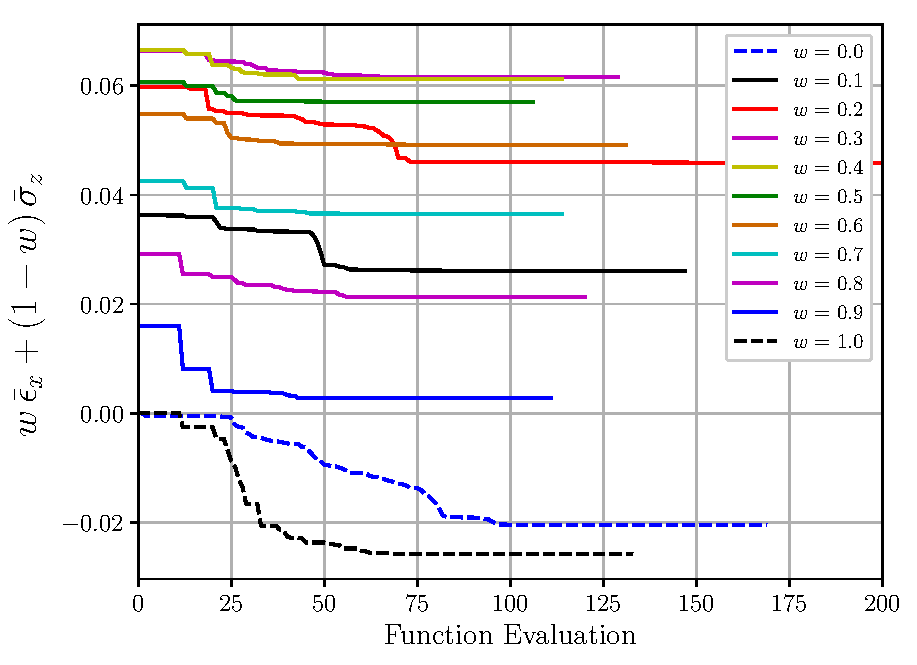
\includegraphics[width=0.9\textwidth]{THPAB155f2}
\end{frame}

\begin{frame}
	\frametitle{Calculating the Pareto Front}
	\textbf{Pareto Front:} the set of parameters for which
	no other point exists that is better with respect to both objectives. 
	Steps to calculate this is basically the same as previous starting points: \\
	\begin{enumerate}
		\item Gather all data from optimization runs and sample
		\item Create finer weight array (i.e. w = np.arange(0, 1.1, 0.001))
		\item Minimize $f(v,w)$ again with finer weights
		\item Plot min points w.r.t $f(v,w)$
	\end{enumerate}
\end{frame}



\begin{frame}
	\frametitle{Approximate Pareto Front}
	\centering
	Trade off between emittance and bunch length
	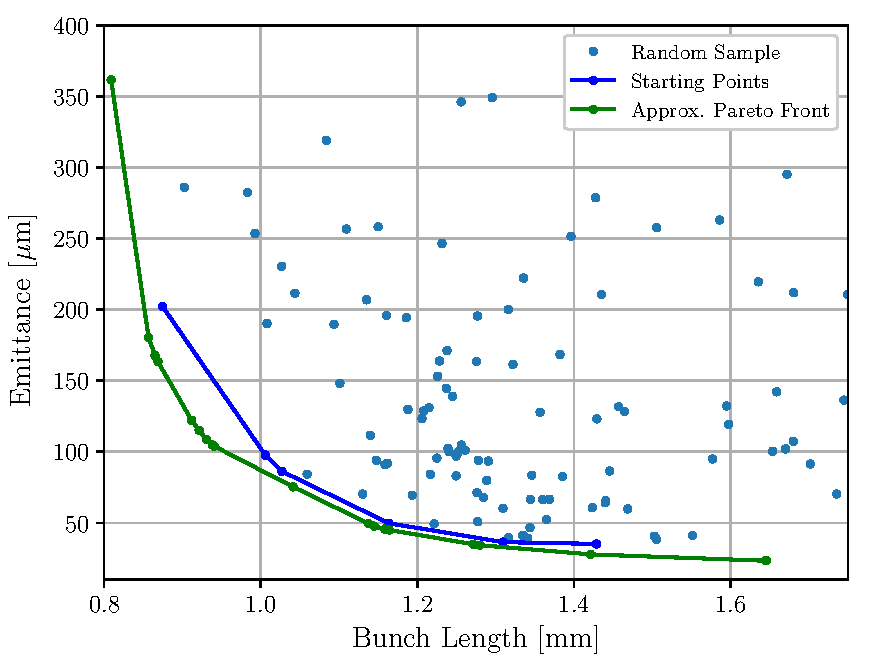
\includegraphics[width=0.9\textwidth]{THPAB155f1}
\end{frame}

\section{Look at Code}
\begin{frame}
	\frametitle{Look at the code...}
	If time permits, let's look at the following in python:
	\begin{itemize}
		\item Random sample
		\item Bobyqa runs
		\item Plotting Pareto Front
	\end{itemize}
	
\end{frame}

\begin{frame}
	\huge Thanks for your time!!\\ 
	\vskip12pt
\end{frame}

\begin{frame}
	\frametitle{Backup: Optimized Gun Results}
	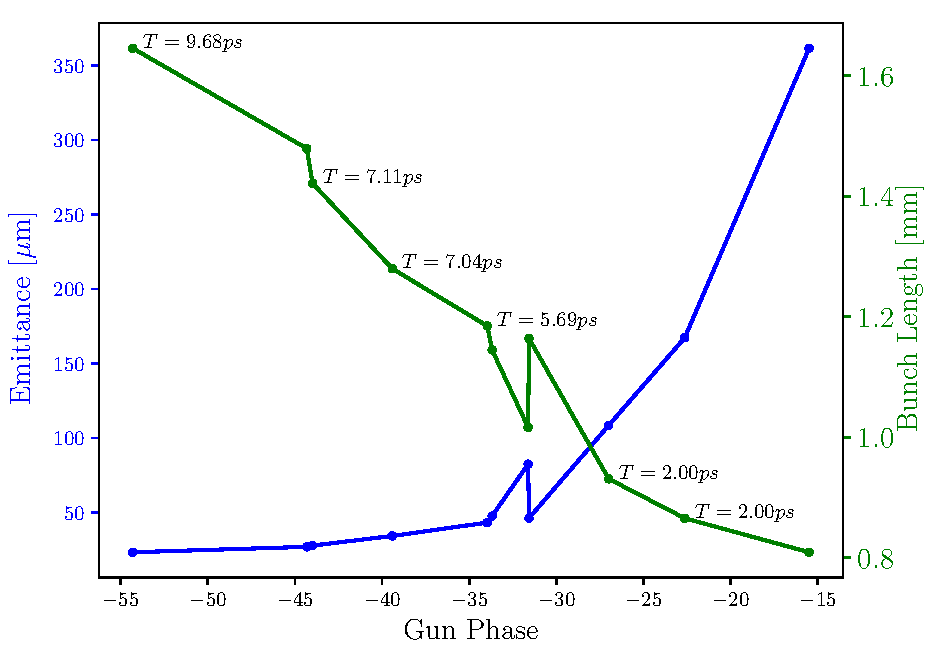
\includegraphics[width=1.0\textwidth]{THPAB155f3}
\end{frame}

\begin{frame}
	\frametitle{Code Features}
	\begin{table}
		\begin{minipage}{\textwidth}
			\begin{center}
				\setcounter{mpfootnote}{\value{footnote}}%
				\renewcommand{\thempfootnote}{\arabic{mpfootnote}}%		
				\begin{tabular}{l c c c}
					\toprule
					\textbf{Feature} & \textbf{ASTRA} & \textbf{GPT} & \textbf{OPAL}\\
					\midrule
					Windows     		& \cmark & \cmark & \xmark \\ 
					Mac         		& \cmark & \cmark & \cmark \\
					Linux       		& \cmark & \cmark & \cmark \\
					Open Source 		& \xmark & \alert \xmark & \color{black!30!green}\cmark \\
					Parallel    		& \alert \xmark\footnote[1]{A parallel version is available at DESY} & \alert \xmark & \color{black!30!green}\cmark \\
					Autophase   		& \cmark & \xmark & \cmark \\
					Adaptive Time Step 	& \xmark & \cmark & \xmark \\
					3D Space Charge 	& \cmark & \cmark & \cmark \\
					Wakefields  		& \cmark & \xmark\footnote[2]{In house module was written at AWA\label{note2}} & \color{black!30!green}\cmark \\
					CSR         		& \alert \xmark & \xmark\textsuperscript{\ref{note2}} & \color{black!30!green}\cmark \\
					\bottomrule
				\end{tabular}
				%\caption{Table caption}
			\end{center}
		\end{minipage}
	\end{table}
	
\end{frame}

\begin{frame}
	\frametitle{Links for pictures}
	Listed in the order they appear:
	\begin{itemize}
		\item GA: https://arxiv.org/pdf/1302.2889.pdf
		\item BOBYQA: https://en.wikipedia.org/wiki/BOBYQA
		\item  
	\end{itemize}
\end{frame}

\end{document}









